\chapter{Introduction}\label{chapter-01}
\section{Motivation: From Fixed-form Structures to Functional Reconfigurable Systems}\label{01-sec-motivation}
Historically, most load-bearing structural systems were conceived as fixed objects that remain in a prescribed configuration throughout their service lives. The geometry, connectivity, and primary function of buildings, bridges, towers, and other civil infrastructure were established during the design phase and remained unchanged after construction. This design philosophy reflected the core priorities of structural engineering, namely, durability, safety, and strength~\cite{schneider2006introduction}. In this context, fixed geometry was not a limitation. It was a practical basis for designing structures with well-defined load paths and predictable service behavior under expected loads.

The persistence of fixed-form structural designs is closely tied to the development of structural engineering itself. Before the rise of modern engineering, resilience in structures was often achieved through practices such as oversizing members, introducing redundancy, and ensuring reparability. With the rise of calculation-based design, these practices were supplemented by methods aimed at achieving safety and durability with greater material efficiency~\cite{hassler2014resilience}. Advances in materials, computational analysis, and construction and fabrication techniques have since expanded the efficiency, scale, and complexity of structural forms~\cite{bechthold2017materials}. Despite these advances, most structures continue to be designed for single use cases, even though modern tools now allow engineers to explore complex geometries and mechanical behavior.

This fixed-form paradigm is becoming increasingly restrictive, especially for a range of emerging applications that require structures to change configuration during storage, deployment, operation, or reuse. Emergency infrastructure, compactly stowable systems, deployable shelters, adaptive load-bearing assemblies, marine structures, and future space-based construction all benefit from systems that can change shape or mechanical response in a controlled manner~\cite{tosun2023analysis, perez2024deployable, foster1987class, thrall2014accordion, yang2024design, churchill2016dynamically, zirbel2013accommodating, miura2009triangles, seo2025review}. In these settings, the utility of a structure depends on transportability, deployability, adaptability, and performance across multiple configurations, in addition to strength and durability in any one configuration. These emerging demands motivate the study of functional reconfiguration, defined here as controlled changes in structural form or mechanical response that preserve, or enhance, the structure's load-bearing purpose. The central challenge, therefore, is to create structures that incorporate reconfigurability without sacrificing stability, load capacity, or application-specific mechanical response.

\section{Current State of Reconfigurable Systems in Engineering}\label{01-sec-reconfigurable-systems}
Over the past century, researchers have developed a wide range of reconfigurable systems for applications that require compact storage for efficient transportation, rapid deployment from stowed configuration, and controlled shape change for functional uses. These systems have largely emerged from automotive, aerospace, mechanical, and robotics engineering, where kinematic performance, packing efficiency, actuation, and adaptability are primary design drivers.

\begin{figure}[!htbp]
  \centering
  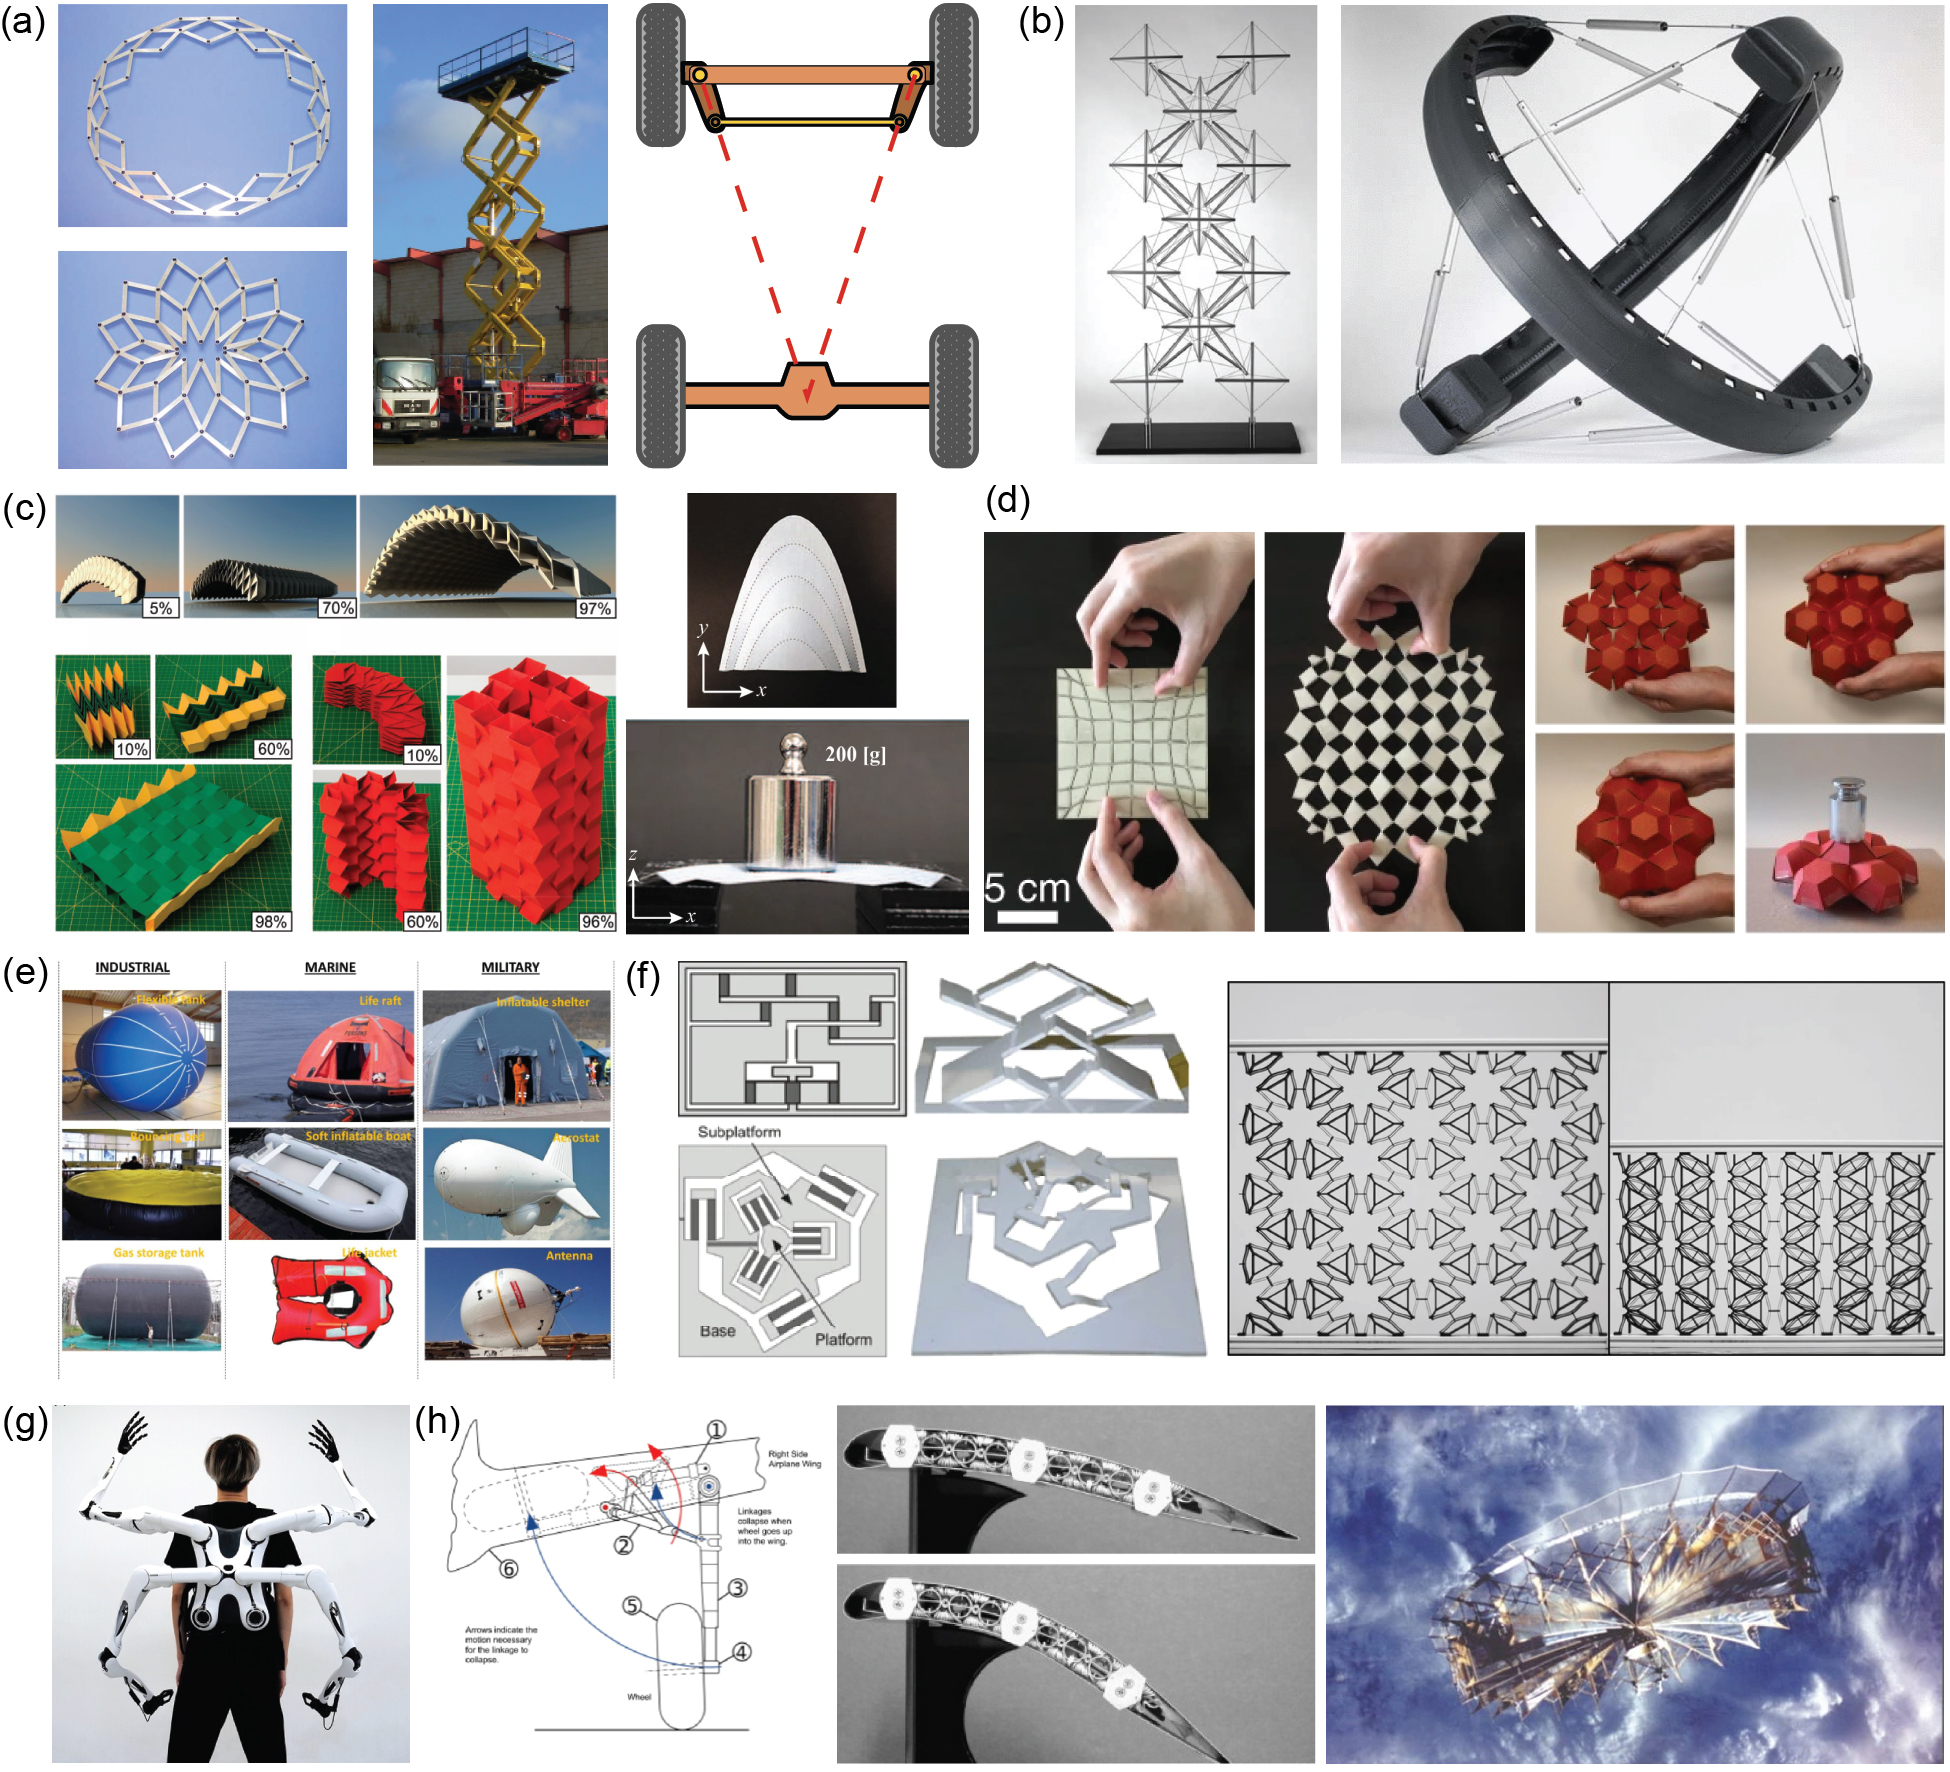
\includegraphics[width=\textwidth]{01-figures/01-01-reconfigurable-structure-examples.jpg}
  \caption{Examples of reconfigurable systems across engineering disciplines. (a) Bar-linked mechanisms: Hoberman linkage~\cite{you2007motion} (left, licensed under CC BY-NC-ND 3.0.), Scissor lift~\cite{knapper2006scissorlift} (middle, licensed under CC BY-SA 2.0 Germany) and Ackermann steering linkage~\cite{bromskloss2010ackermann} (right, licensed under CC BY-SA 3.0); (b) Tensegrity structures: planar tensegrity mast~\cite{snelson2012art} (left, adapted with permission from Sage Publications) and sperical tensegrity robot~\cite{bohm2016spherical} (Copyright \copyright{} 2016, IEEE); (c) Origami tubes for stiff columns, bridges and domes~\cite{filipov2015origami} (left) and curved-crease origami~\cite{woodruff2021curved} (right, adapted with permission from Springer Nature); (d) Kirigami systems: planar auxetic kirigami~\cite{choi2019programming} (left, adapted with permission from Springer Nature) and pop-up kirigami domes~\cite{redoutey2021pop} (right, adapted with permission from Elsevier); (e) Membrane based inflatable systems~\cite{mandlekar2022review} (licensed under CC BY-NC-ND 4.0); (f) Compliant mechanisms~\cite{howell2013compliant} (adapted with permission from Springer Nature) and multistable metamaterials~\cite{zhang2019energy} (licensed under CC BY 4.0); (g) Robotic arms~\cite{yamamura2023social} (licensed under CC BY 4.0); and (h) Aerospace systems: aircraft landing gear~\cite{dtom2009landinggear} (left), shape morphing wings~\cite{sofla2010shape} (middle, adapted with permission from Elsevier) and mesh reflector antenna deployed in orbit~\cite{santiago2013advances} (right, adapted with permission from Springer Nature).}\label{fig-reconfigurable-structures}
\end{figure}

The resulting body of literature spans many distinct families of systems. Mechanical linkages, including Scissor mechanism and Ackerman linkage shown in Fig.~\ref{fig-reconfigurable-structures}\,(a), use connected bars and rotational joints to produce prescribed motion, expansion, and controlled deployment. Tensegrity assemblies consist of isolated compressive struts within a network of prestressed tensile tendons. The balance between these compressive and tensile members enables the creation of lightweight, deployable space masts and towers, as shown in Fig.~\ref{fig-reconfigurable-structures}\,(b). Origami-inspired systems use folding of flat sheets along prescribed crease patterns to generate complex, three-dimensional structures. Origami principles help create structures with intricate surface topologies, architected mechanical responses, and enable compact storage, deployment, and reconfigurability, as shown in Fig.~\ref{fig-reconfigurable-structures}\,(c). Kirigami systems extend the idea of origami further by incorporating strategically placed cuts or slits into thin sheets of material. These cuts help generate auxetic behavior, enhanced flexibility, tunable mechanical properties, and large shape transformations that are difficult to achieve solely through folding, as shown in Fig.~\ref{fig-reconfigurable-structures}\,(d). Pneumatic and membrane-based structures use thin flexible sheets that gain shape and stiffness through internal pressure, prestress, or supporting boundary elements, as shown in Fig.~\ref{fig-reconfigurable-structures}\,(e). Compliant, multistable, and metamaterial systems use elastic instabilities and geometric nonlinearities to program motion, dissipate energy from external loads, or maintain multiple stable states, as shown in Fig.~\ref{fig-reconfigurable-structures}\,(f). Robotic and aerospace systems combine structural components with actuation, sensing, and control to interact with their environment, as shown in Fig.~\ref{fig-reconfigurable-structures}\,(g) and (h).

Despite significant progress, incorporating deployable and reconfigurable systems into conventional large-scale load-bearing structures remains challenging. Civil structures must satisfy strict requirements for stiffness, strength, stability, constructability, reliable connections, and predictable load transfer under prescribed loading conditions. Many reconfigurable systems provide effective mechanisms for shape change, but their changing geometry, complex joints, and material assumptions pose challenges during large-scale implementation. For instance, origami-inspired systems offer powerful ways to transform flat sheets into complex three-dimensional forms. However, at large scales, the thin-sheet mechanics of origami must be adapted to incorporate finite-thickness panels to ensure robust load transfer between components. Even with thickness-accommodation strategies, these systems can develop unintended moments, localized strains, and complex hinge behavior along creases. Compliant mechanisms, multistable systems, and metamaterials provide useful strategies for programmed deformation and energy absorption from external loads. However, many remain tied to small-scale architectures, specialized materials, or unit-cell-level behavior, which do not directly translate to large structural assemblies with conventional members, joints, and supports. Thus, existing systems offer many principles for creating deployable and reconfigurable systems, but far fewer methods for incorporating those principles into established structural topologies that engineers already understand and trust. The next section uses this distinction to define the specific research problem addressed in this dissertation.

\section{Problem Statement: Integrating Reconfigurability into Existing Structural Forms}\label{sec-problem-statement}
The preceding section shows that reconfigurable systems have been studied across many fields. However, many of these systems are designed with a bottom-up philosophy, in which the unit cell is repeated to create a larger system. This dissertation considers the inverse problem of introducing reconfigurability into an existing structural topology without losing the structural function that made the original topology useful.

The central gap is the lack of generalized frameworks for transforming existing structural topologies into reconfigurable systems. Conventional structures such as trusses, frames, and hulls are typically designed to withstand prescribed loads in a fixed configuration. In contrast, reconfigurable systems must satisfy two coupled requirements: they must move between useful configurations and retain predictable mechanical behavior during and after reconfiguration. Existing studies often address one of these requirements in isolation. Mechanism-based studies emphasize motion, while conventional structural design emphasizes load resistance. The unresolved problem is how to combine these requirements in a systematic way.

This gap has three parts. First, there is a need for design methods that begin with conventional structural topologies, rather than with specialized reconfigurable mechanisms. Second, there is a need for analysis tools that can capture the kinematics, load demands, and stability of the resulting systems through large geometric changes. Third, there is a need to understand how added mechanical features, such as rotational stiffness and nonlinear hinge behavior, can turn reconfiguration from a geometric capability into a functional structural response.

We address this broad problem in the context of two structural systems in this dissertation. The primary focus is on truss systems due to their simple and well-defined geometry, connectivity, and load paths. This makes trusses an appropriate platform for studying how static structural topologies can be transformed into reconfigurable systems. The dissertation then extends this broader philosophy to ship hulls, where curved origami principles are used to introduce compact storage, rapid deployment, and on-demand shape-morphing behavior within an established hull form. These two contexts differ in geometry and application. However, they share a common objective: to move from isolated reconfigurable mechanisms to functional reconfigurable structural systems.

\section{Objectives of the dissertation}\label{01-sec-objectives}
This dissertation addresses the central gap identified in the previous section through four objectives.

\noindent{}\textbf{Objective 1: Develop a framework for transforming static trusses into reconfigurable systems.}\\
We develop a framework for transforming static truss designs into reconfigurable systems using principles of planar quadrilateral linkages. The framework introduces kinematic degrees of freedom into selected truss units, enabling the transformed systems to change shape while preserving the primary load paths, stiffness, and peak load capacity of the original designs. We also develop fabrication strategies that allow the transformed systems to deploy as intended without member interference or loss of strength due to out-of-plane moments.

\noindent{}\textbf{Objective 2: Develop computational tools for kinematic and mechanical analysis.}\\
We develop computational tools to evaluate the kinematic and structural response of the reconfigurable trusses. The kinematic tool uses a sequential actuation framework to simulate deployment paths and quantify the packing efficiency of the transformed systems. The structural tool uses a geometric nonlinear analysis framework with axial bar and torsional spring elements to evaluate actuation load demands, behavior during load reversal, and structural response during large deformations.

\noindent{}\textbf{Objective 3: Incorporate programmed hinge behavior into reconfigurable trusses for functional applications.}
We develop programmed rotational hinges that introduce prescribed nonlinear moment-rotation behavior into reconfigurable truss systems. This objective combines a physical hinge design based on magnetic interactions between alternating-polarity magnets with nonlinear torsional spring models that capture bistable and multistable rotational responses. We show that these programmed hinges can assign multiple stable states to independent degrees of freedom in reconfigurable trusses, enabling functional applications such as reusable impact absorption infrastructure.

\noindent{}\textbf{Objective 4: Broaden the framework beyond civil truss systems through curved-crease origami hulls.}\\
We extend the dissertation's philosophy beyond civil structures by using curved-crease origami principles to obtain shape-morphing ship hulls. This objective develops flat-foldable and rapidly deployable hull systems that match conventional planing hull geometries and morph shape for on-demand tunability of hydrodynamic performance. Through this extension, we show that reconfigurability can also be used to rethink established structural forms in naval architecture to achieve functional benefits, such as adaptable hydrodynamic performance.

\section{Organization of the Dissertation}\label{01-sec-organization}
The dissertation is organized as follows to address the objectives described in the previous section:

\textbf{Chapter~\ref{chapter-02}} introduces a method for transforming static trusses into reconfigurable systems. This method uses Grahsof's flat-foldability criterion for planar quadrilateral linkages to strategically introduce a new node in every triangular unit of a given truss. These added nodes convert triangular units into flat-foldable quadrilateral linkages, thereby introducing kinematic degrees of freedom that enable global reconfigurability. A general workflow is presented for applying these transformations to most single-chorded truss designs, and it is supported by a sequential kinematic analysis framework to study the deployment behavior of the resulting systems. This workflow is first demonstrated on traditional truss designs and then extended to topology-optimized trusses with arbitrary geometries, to highlight its broader applicability. The chapter also presents experimental structural analysis of proof-of-concept prototypes to demonstrate fabrication feasibility and to show that the transformed systems retain load-bearing capacity and stiffness of the original designs.

\textbf{Chapter~\ref{chapter-03}} develops a Three-node Torsional Spring (3NTS) element to introduce rotational stiffness at the folding joints of the reconfigurable trusses developed in Chapter~\ref{chapter-02}. The chapter presents a first-principles mathematical formulation of a torsional coil spring element and its implementation within a nonlinear structural solver. The formulation is validated against analytical solutions for two benchmark examples, demonstrating its ability to capture structural instabilities associated with elastic buckling. The chapter then shows how torsional springs can be integrated into reconfigurable trusses to provide functional benefits such as resistance to load reversal, controlled path-dependent deployment, and energy absorption under external loading.

\textbf{Chapter~\ref{chapter-04}} extends the 3NTS formulation from Chapter~\ref{chapter-03} by introducing hinge-level nonlinear constitutive models for bounded rotation, magnetic multistability, and idealized bistability. These models enable the simulation of programmable mechanical response in reconfigurable trusses, including sequential deployment and path-dependent multistability. This capability establishes a foundation for future functional applications of reconfigurable trusses such as reusable infrastructure for impact-energy management.

\textbf{Chapter~\ref{chapter-05}} broadens the perspective of the dissertation by extending the transformation of static structural topology beyond civil engineering and into naval architecture. In this chapter, the focus shifts from reconfigurable truss systems to shape-morphing hull structures inspired by curved-crease origami. The chapter develops curved-crease-origami-inspired planing hulls that can be deployed rapidly from flat sheets, match the shape and therefore, hydrodynamics of conventional planing hulls, and utilize active folding to change shape and tune hydrodynamic performance of the hull on demand. A proof-of-concept prototype is also presented, together with a discussion of the steps required for real-world implementation.

\textbf{Chapter~\ref{chapter-06}} summarizes the main contributions of the dissertation, discusses its limitations, and outlines directions for future research.

Three appendices are included to provide additional background for the analytical tools and methods used throughout the dissertation.

\textbf{Appendix~\ref{01-appendix-seq-kinematics}} presents the mathematical formulation for the positional analysis of planar quadrilateral linkages, which serves as the basis of the sequential kinematic analysis framework used to study deployment of reconfigurable trusses. This appendix also includes the positional analysis of the special six-bar linkage case discussed in Chapter~\ref{chapter-02}, together with a note on interpreting the percentage of actuation of each kinematic degree of freedom in the reconfigurable truss systems.

\textbf{Appendix~\ref{02-appendix-truss-videos}} contains the supplementary videos of fabricated reconfigurable truss prototypes and their load-tests discussed in Chapter~\ref{chapter-02}, to demonstrate failure type and load-carrying capacities.

\textbf{Appendix~\ref{03-appendix-powersea}} describes the theoretical basis of the Powersea software used for the hydrodynamic analyses of planing hulls in Chapter~\ref{chapter-05}. This appendix briefly outlines the \textit{low-aspect-ratio strip theory} used in the software, states the key assumptions, and explains why this approach is suitable for comparative hydrodynamic studies of curved-crease origami and conventional planing hulls.